\section{UV Laser System}
\label{sec:laser}
%{\it{Igor}}

The knowledge of the electric field inside the drift volume of a \lartpc is a necessary aspect for performing subsequent event reconstruction. Distortions of particle tracks due to field non-uniformities affect the accuracy of the particle momentum reconstruction based on multiple scattering.  Deviations from a uniform drift field may arise mainly due to accumulation of positive argon ions in the drift volume. These ions are produced by ionizing particles from neutrino interactions, as well as by cosmic rays. While electrons produced by ionizing particles are quickly (within few milliseconds) swept towards the readout system, ions have significantly lower mobility. Their drift velocity in the MicroBooNE detector at nominal drift field is of the order of 0.8 cm/s. The rate of cosmic muons in the \lartpc volume is estimated to be 11,000 muons/s within the active volume (assuming a cosmic rate of 200 muons/m$^2$/s through a horizontal plane at the earth's surface and 63 muons/m$^2$/s through a vertical plane), traversing a combined length of 1.9$\times$10$^4$ m through the liquid argon.  Assuming that cosmic muons are minimum-ionizing (2.1 MeV/cm) and produce 23.6 eV per ion pair, positive ion charge is produced at a rate of 2.8$\times$10$^{-8}$ C/s in the MicroBooNE TPC. These ions are continuously neutralized at the cathode. The resulting charge distribution in equilibrium is shown in figure \ref{Ions}. Such accumulated space charge leads to noticeable distortion of the drift field and, consequently, to deviations of reconstructed track coordinates by up to 10cm (see figure \ref{Coordinates}).  The ion drift velocity is comparable to local argon flow velocities, produced by global argon recirculation flow and thermal convection. Therefore the distribution of positive space charge inside the drift volume may be not only nonuniform (figure \ref{Voirin}), but also non-stationary.

\begin{figure}[htb]
\centering	
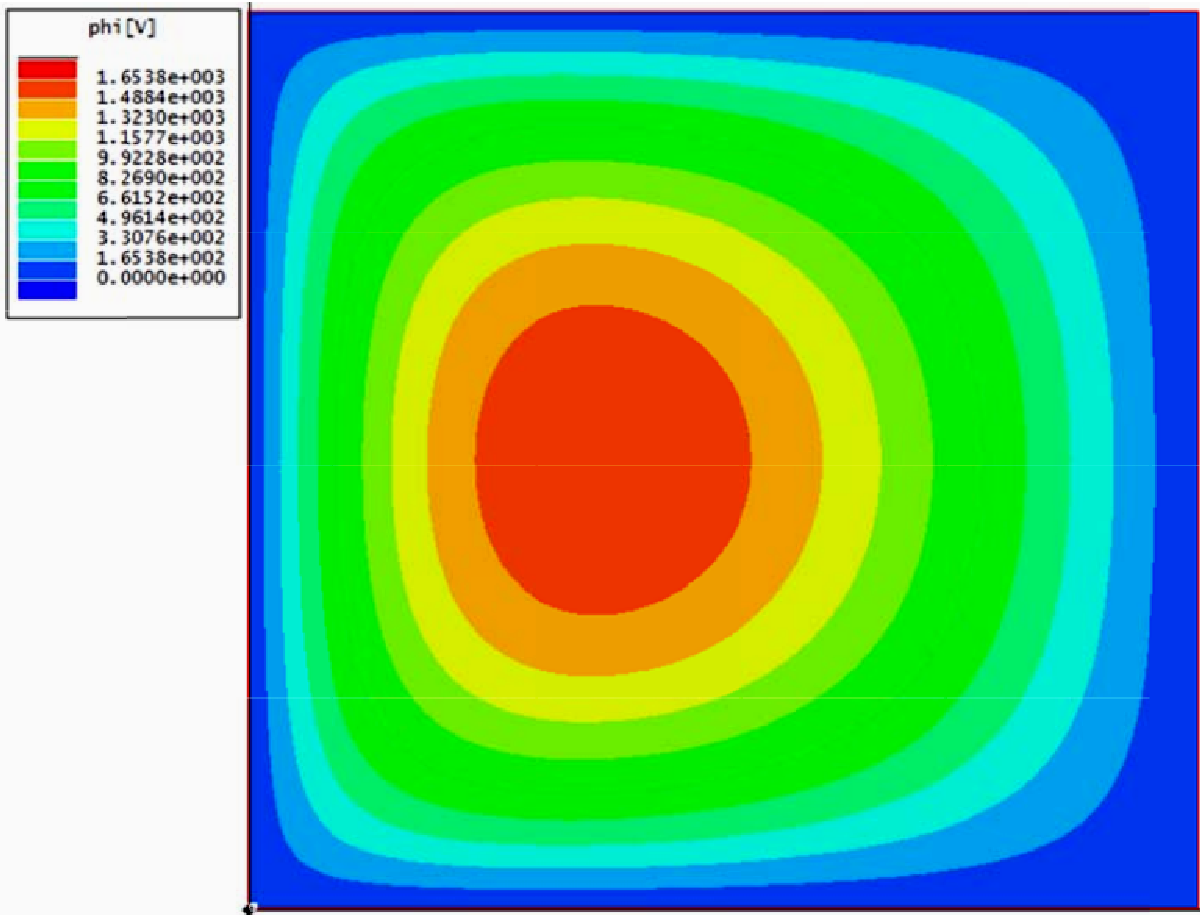
\includegraphics[width=0.8\textwidth]{figures/Potential.pdf}
\caption{Distorting potential distribution due to positive space charge in equilibrium in the MicroBooNE detector.}
\label{Ions}
\end{figure}

\begin{figure}[htb]
\centering	
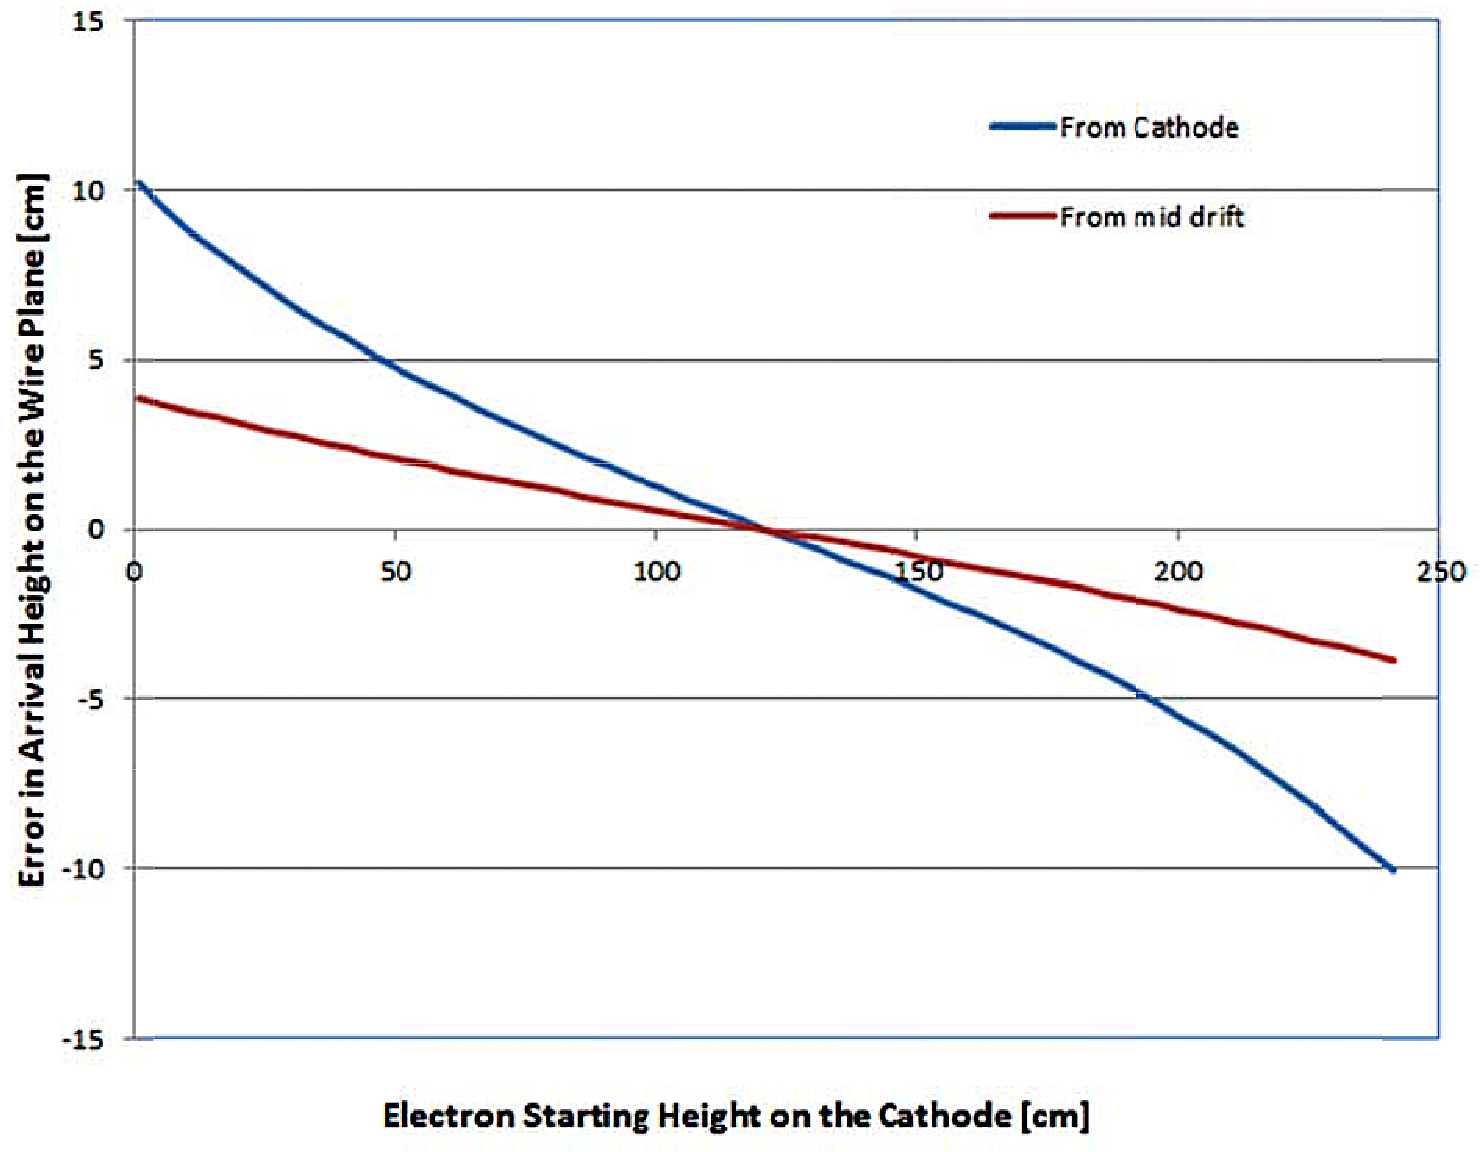
\includegraphics[width=0.8\textwidth]{figures/Coordinate.pdf}
\caption{Deviation of a crossing track from its true coordinates due to positive ion space charge.}
\label{Coordinates}
\end{figure}

\begin{figure}[htb]
\centering	
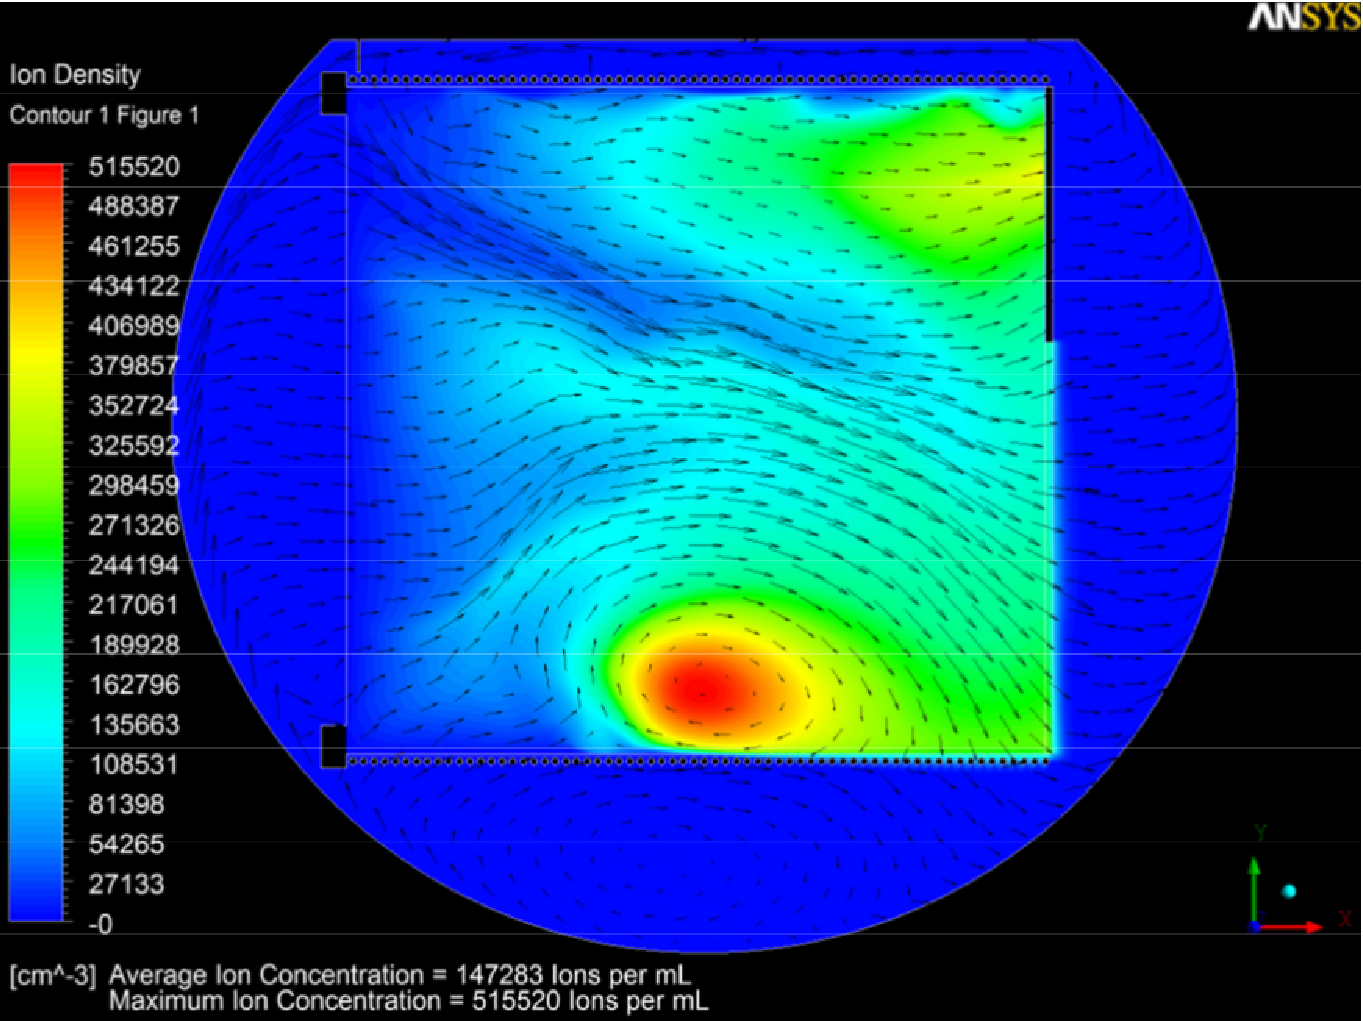
\includegraphics[width=0.8\textwidth]{figures/Voirin.pdf}
\caption{Distribution of the positive space charge in presence of argon circulation.}
\label{Voirin}
\end{figure}


A nonuniform drift field in the \lartpc leads to bending of initially straight tracks of high-momentum ionizing particles. In principle, a set of events from such particles allows for the reconstruction of the field in any small region of the \lartpc drift volume, using the systematic apparent curvature of tracks at different angles passing through that region. In practice, the rate of such events from cosmic muons is too low to acquire sufficient statistics in reasonable time. A method to generate straight ionization tracks at a defined location in liquid argon is described in \cite{Badhrees:2010}. A collimated photon beam from a pulsed UV laser with $\lambda$=266~nm can ionize liquid argon via multi-photon absorption. The resulting ionization track is straight, characterized by low electron density, therefore featuring little charge recombination loss, unlike cosmic muon tracks. Laser tracks are also free from $\delta$-electrons, which complicate track reconstruction in the case of muons. The method was successfully exploited in the Argontube long drift \lartpc \cite{Badhrees:2012-argontube,Ereditato:2013-argontube,Zeller:2013-argontube} to derive the non-uniformity of the electric field along its 5~m long drift volume (see \cite{Ereditato:2014-argontubedrift}). The MicroBooNE \lartpc requires a set of such tracks in order to cover the whole sensitive volume to reconstruct field distortions. Tracks are generated one at a time by steering a pulsed laser beam with the use of a custom-designed opto-mechanical feedthrough (see \cite{Ereditato:2014-laser}). The pulse rate of the laser generator is 10~Hz. This allows production of a minimum required set of 100 tracks within one minute (taking into account steering time). Details of this solution are described in the following sections.

\subsection{UV Laser Calibration}
In order to unambiguously reconstruct a drift field vector at any point within the detector fiducial volume, a minimum of two ionization tracks are required to cross in the region of interest. The total number of crossing points is determined by the required reconstruction granularity. In MicroBooNE the initial scenario is to acquire 100 tracks from each direction, producing a reconstructed 3-D map with voxels that are approximately 10x10x50 cm$^3$ in volume. This map provides a rough picture of the space charge distribution. Depending on the results of this measurement, areas of interest can be studied in more detail. Repetitive study of small volumes may reveal dynamics in the space charge distribution due to turbulent circulation, and should further inform an optimized scenario for a standard UV laser calibration procedure.  

An algorithm of drift field calibration utilizes an input array of detector events with one straight ionization track in each element of the array. The result of the calibration is a coordinate correction map, to be applied to each track, which converts apparently curved track images back to the true coordinate system where they are straight. The algorithm is iterative with an optimizable iteration step and required accuracy. An example of simulated reconstruction in 2-D space is depicted in figure \ref{Reco}, showing that the magnitude of the field distortions is reduced from 10~cm down to several millimeters in 99\% of the detector volume.


\begin{figure}[htb]
\centering	
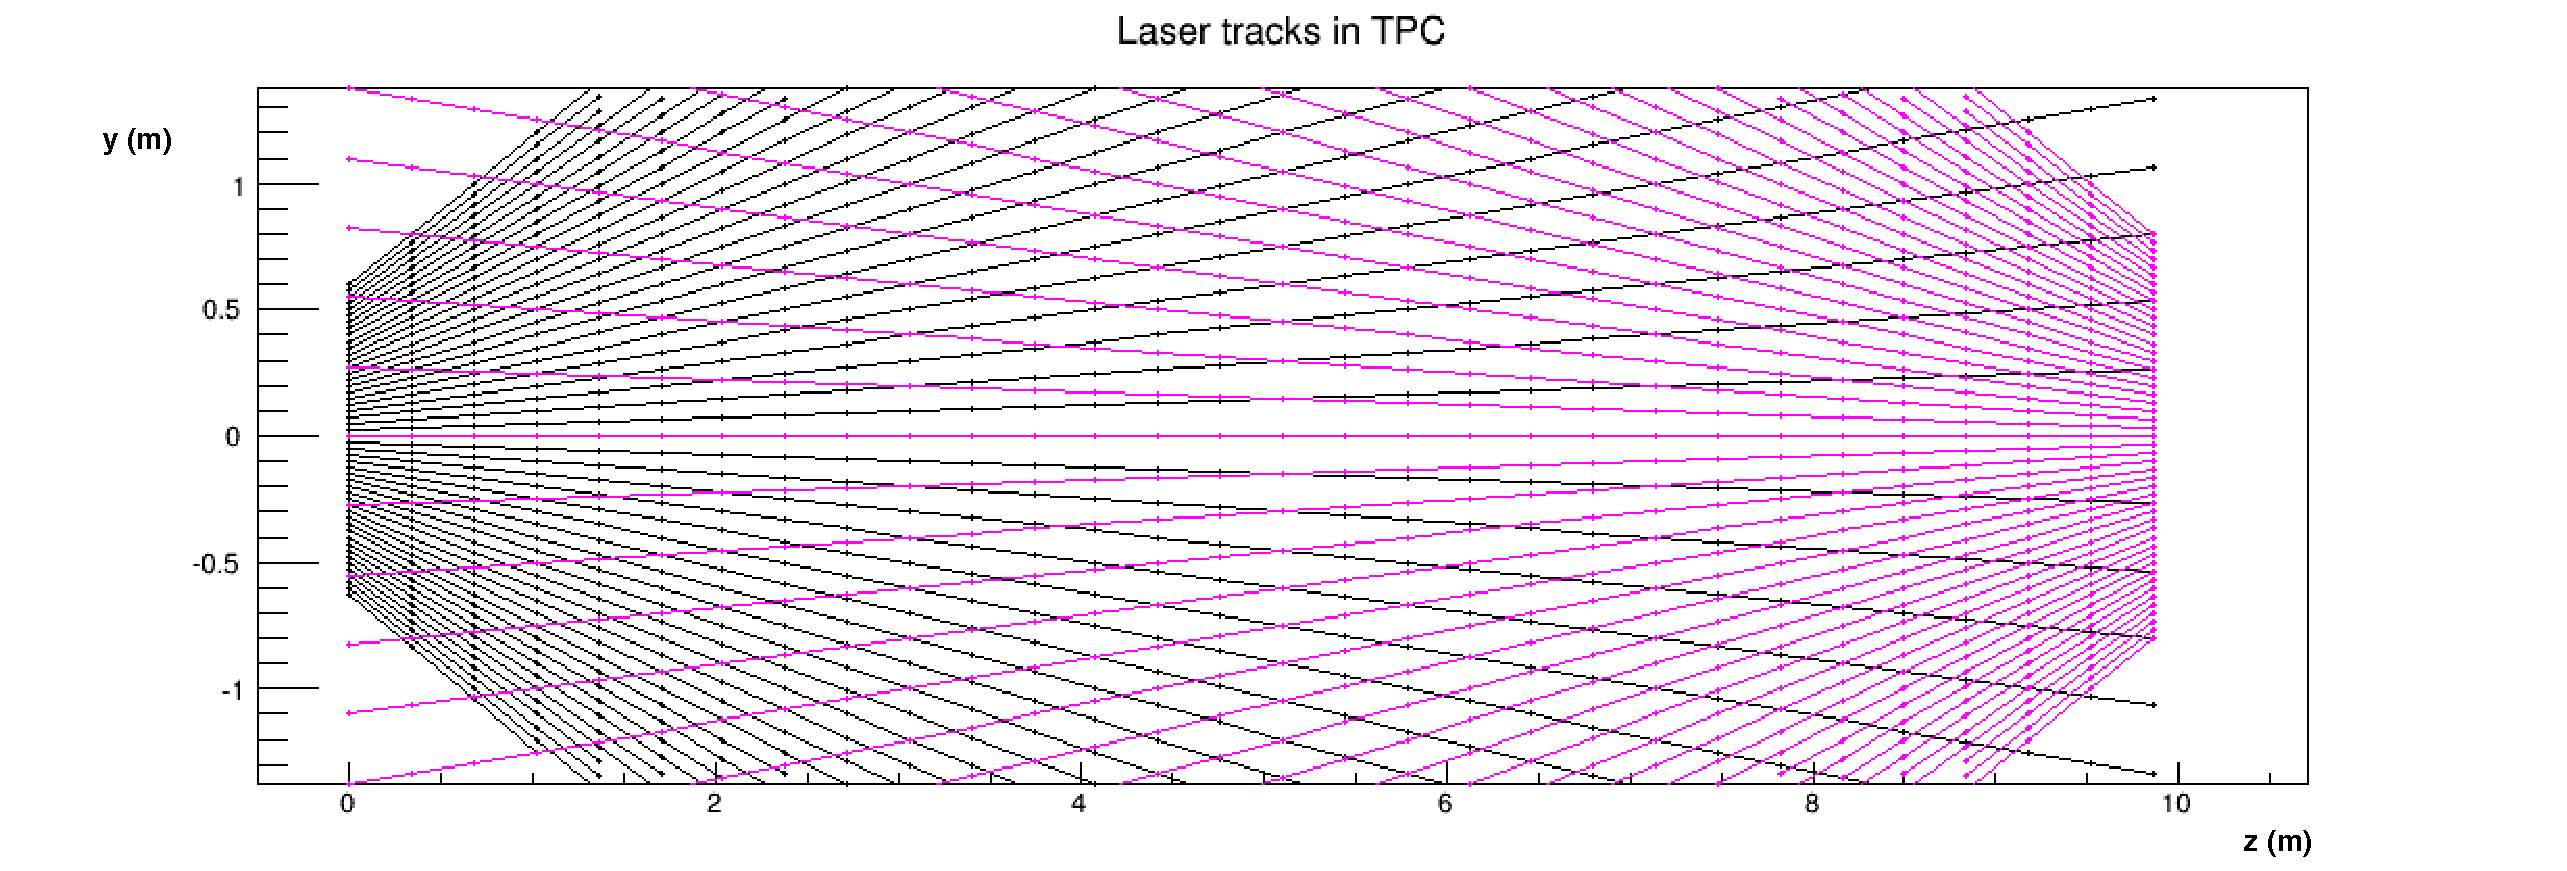
\includegraphics[width=0.98\textwidth]{figures/Original_Tracks.pdf}
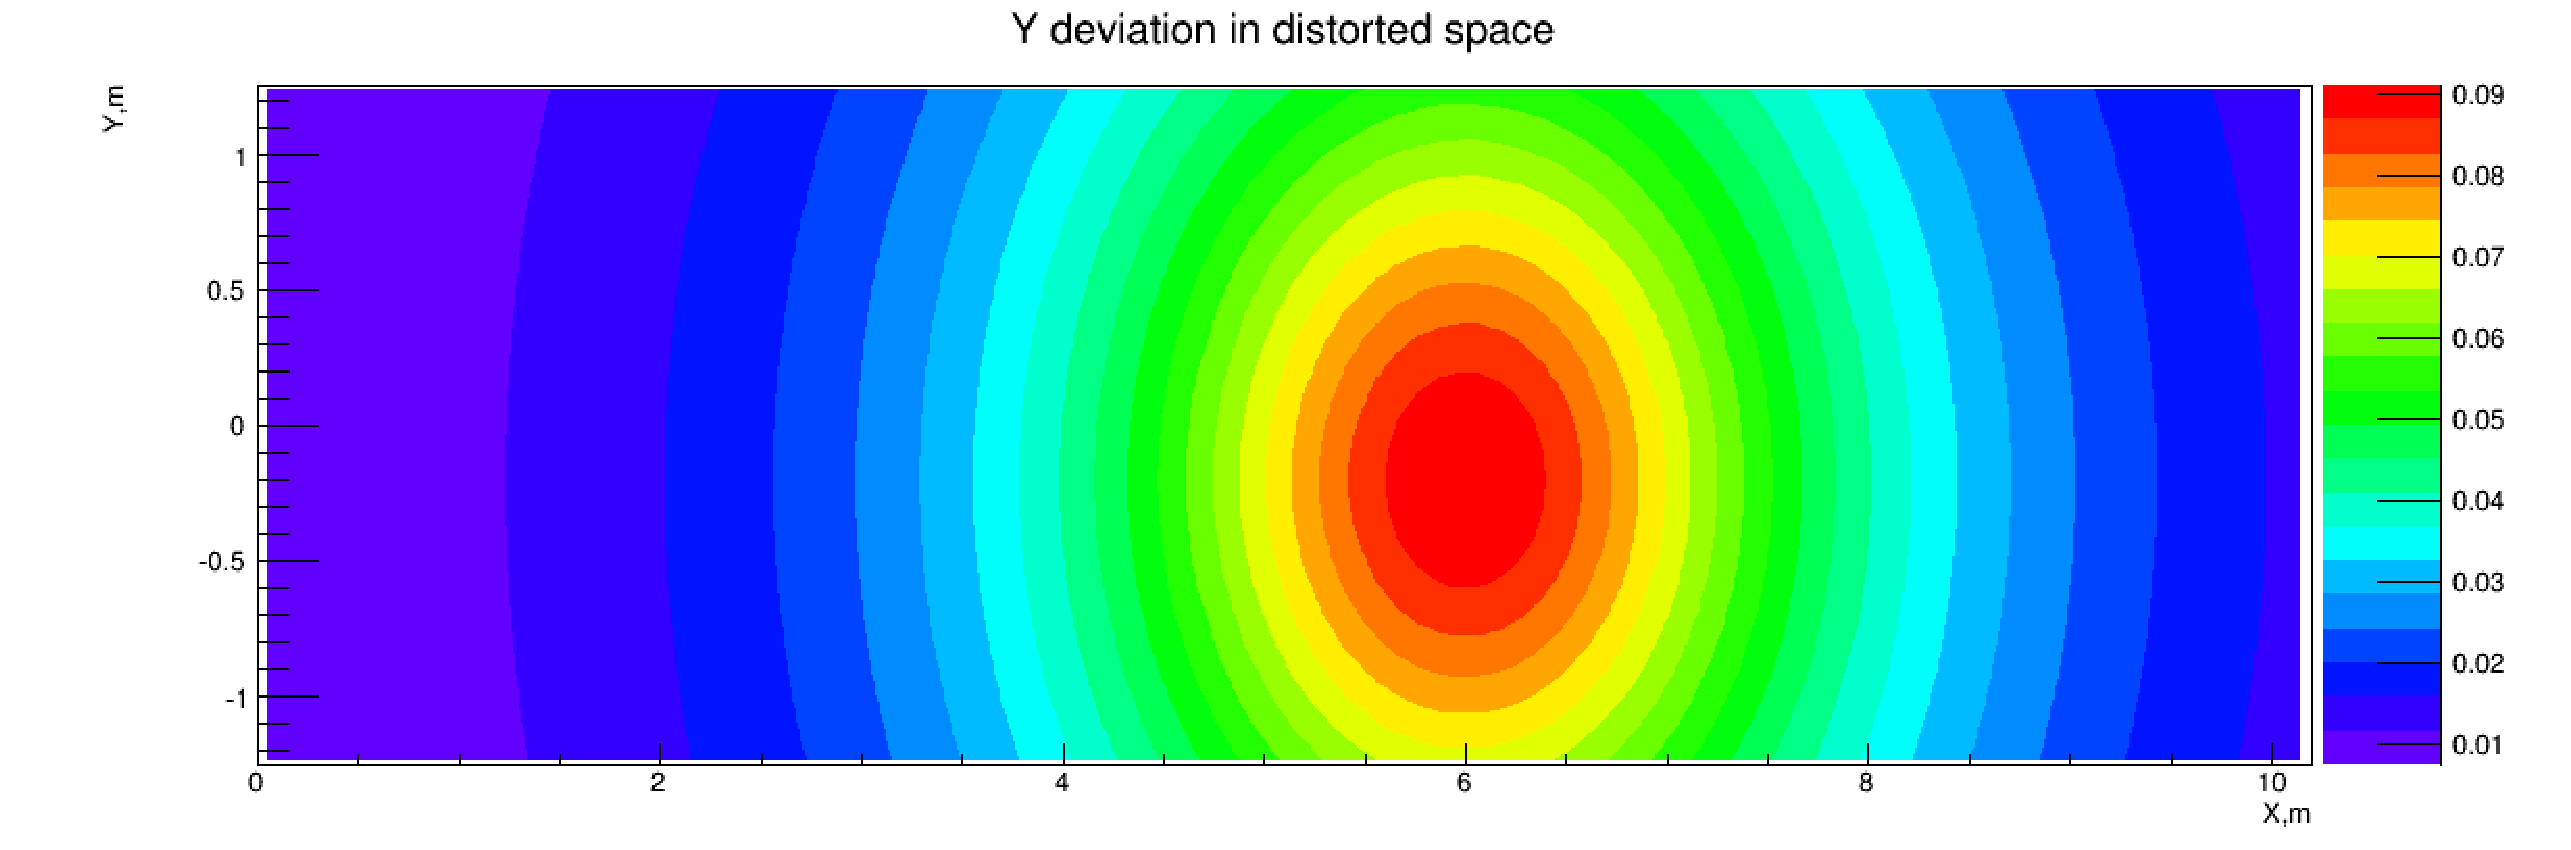
\includegraphics[width=0.98\textwidth]{figures/Ydev.pdf}
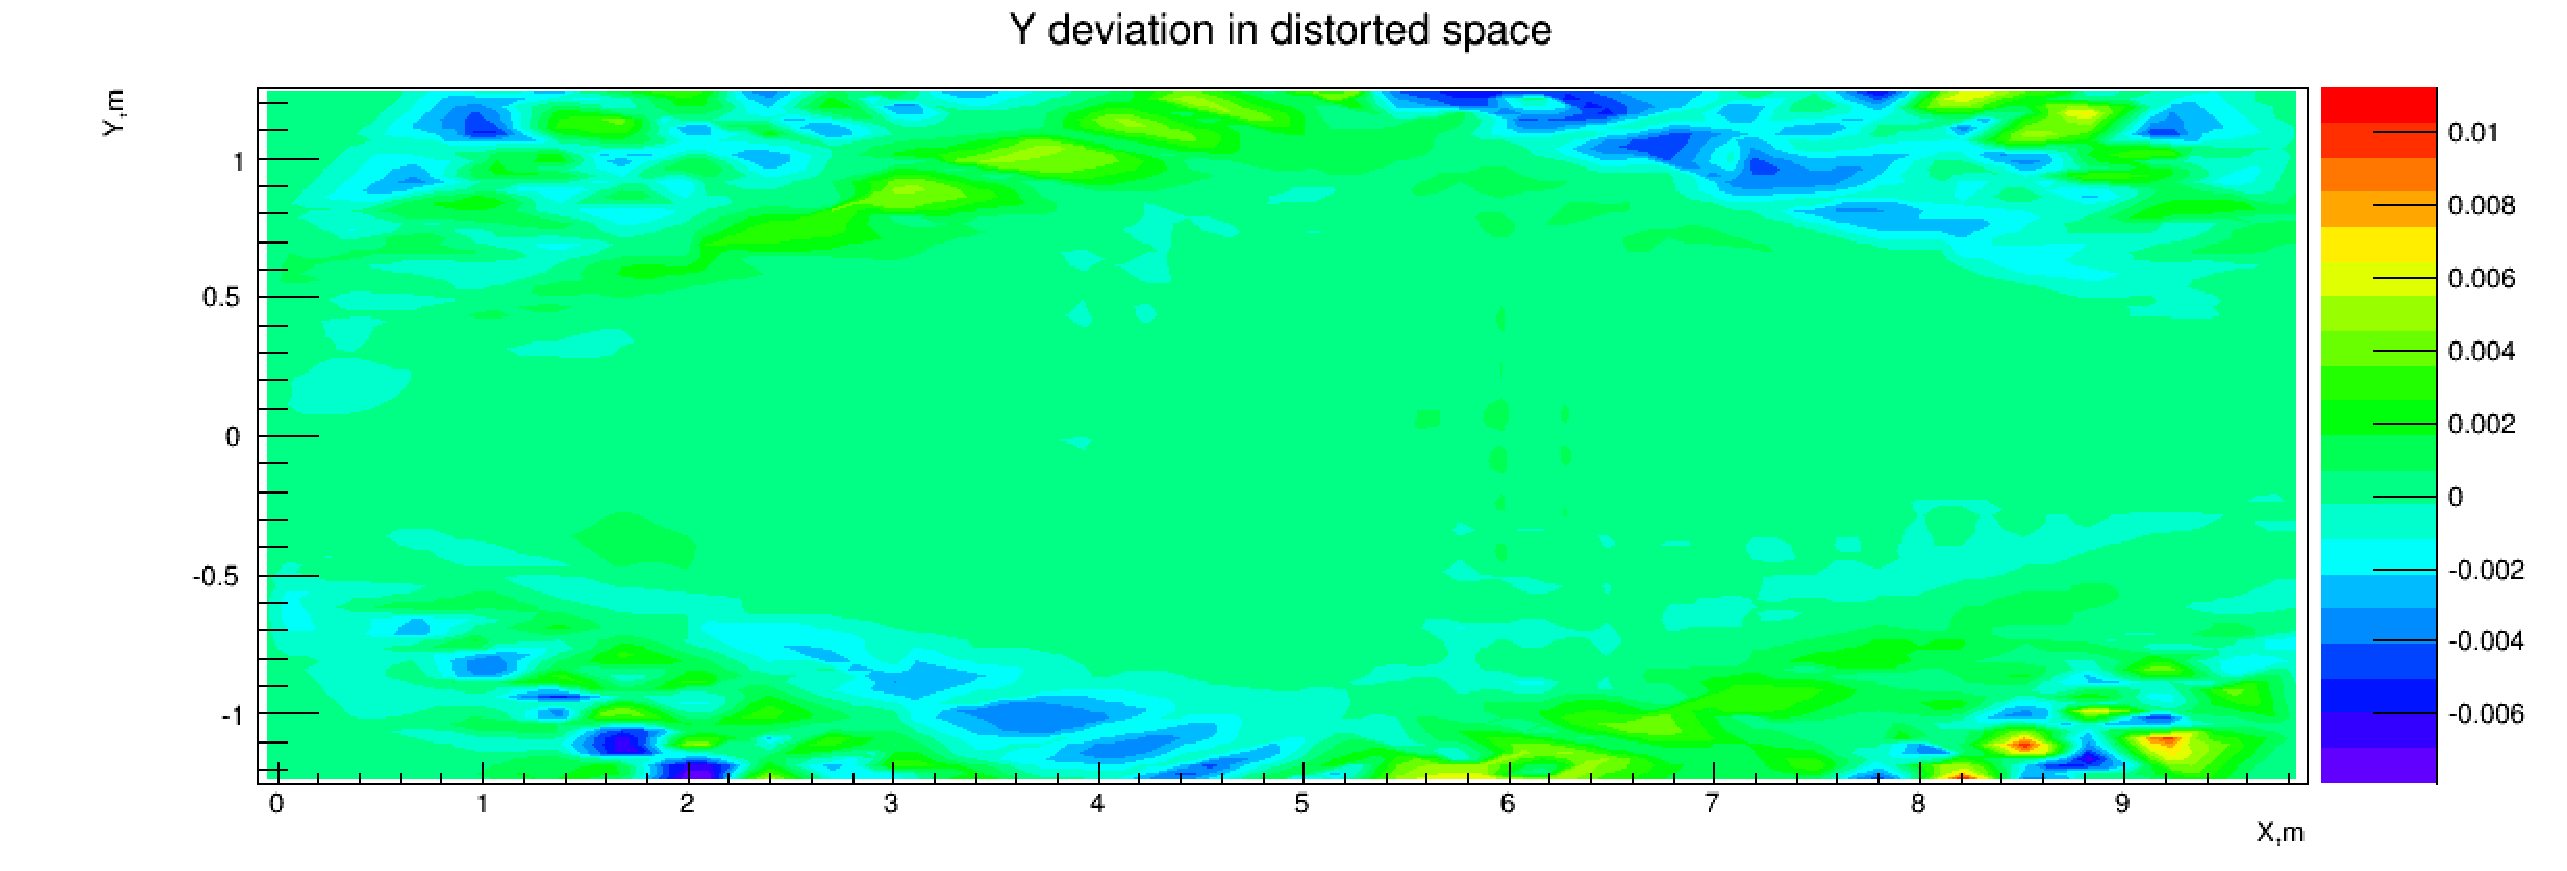
\includegraphics[width=0.98\textwidth]{figures/Yresidual.pdf}
\caption{Top: Simulated true laser beam trajectories in the detector; Middle: map of Y coordinate of track deviation under influence of non-uniform electric field; Bottom: residual map of reconstructed track Y-coordinates versus true ones.} 
\label{Reco}
\end{figure}


\subsection{Laser Source and Optics}
A Nd:YAG laser emitting light at a wavelength of 1024~nm is used as the primary light source \cite{continuum}. Inside the laser head, nonlinear crystals are installed in the beam line for frequency doubling and summing, resulting in a wavelength of 266~nm needed for ionization of liquid argon. For this wavelength, the Nd:YAG laser is specified to produce an output energy of 60~mJ for each 4 to 6~ns long pulse and a horizontal polarization. The maximal repetition rate is 10~Hz; the beam has a divergence of 0.5~mrad.

An optical table, as seen in figure \ref{fig:optics}, was developed to introduce the necessary parts in a stable and compact environment. With regard to the operation of the optical table on MicroBooNE, the parts were chosen to be accessible remotely where necessary. The emitted laser beam contains not only ultraviolet light but also all other harmonics generated in the crystal and the primary light of 1024~nm. Dichroic Mirrors optimized to reflect only wavelengths in the UV region are used to filter higher wavelengths out. To absorb the transmitted wavelength behind the mirrors, glass-ceramic plates are installed. The beam leaving the laser head is reflected by the first $45^{\circ}$-mirror into an attenuator. For optical adjustment and verification of the non-visible UV-beam, a green alignment laser is placed behind this mirror and adjusted such that its path is coincident with the UV-laser beam. In the attenuator (Altechna Wattpilot) a turnable $\lambda/2$-plate enables rotation of the orientation of the laser beam polarization. Behind the attenuator two parallel plates are installed such that the angle of the incident beam matches the Brewster angle of the reflector. Modulating the polarization of the beam adjusts the intensity of the reflected beam. After the attenuator an aperture is put in the optical path of the beam to control the beam diameter. The last part in the beam line is a remotely-controllable mirror mount (Zaber T-OMG), which directs the beam to the laser feedthrough on the cryostat. A photodiode (Thorlabs DET10A/M), which is sensitive in the ultraviolet region, detects the scattered light when a laser pulse is fired.  Its signal is then used as a trigger for data taking. Both the UV-laser head and the optical table are mounted on a 15~mm thick aluminum plate.

\begin{figure}%
    \centering
    \subfloat[Optical Table]{{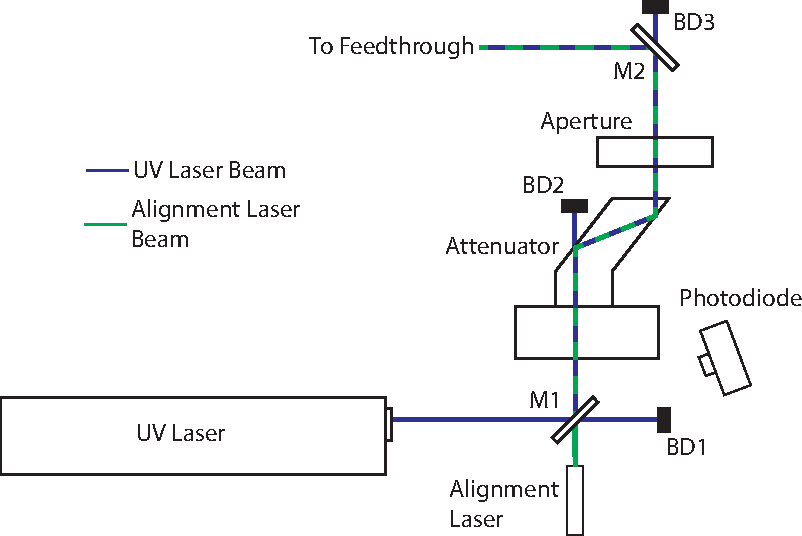
\includegraphics[width=.6\textwidth]{figures/optics.pdf} }}%
    \qquad
    \subfloat[Side View]{{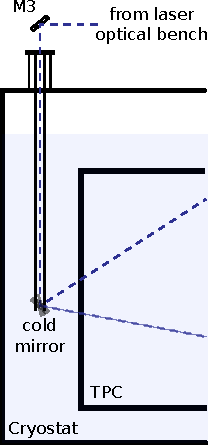
\includegraphics[width=.2\textwidth]{figures/feedthrough2.pdf} }}%
    \caption{(a) A schematic drawing (not to scale) of the components used for laser beam configuration.  An alignment laser (visible light) is introduced along the UV-laser path at the first dichroic mirror (M1), such that the paths overlap. In the attenuator the UV-laser beam intensity can be adjusted to the desired level, and the diameter of the beam is controlled by an aperture. A motorized mirror (M2) deflects the light into the direction of the feedthrough. Beam dumps (BD) are installed behind all mirrors to absorb the non-reflected laser light. (b) Side view of the cryostat indicating the mirror support structure with respect to the LArTPC.}%
    \label{fig:optics}%
\end{figure}


\subsection{Steering System}
One of the main challenges of the laser calibration system is the introduction of a steerable laser beam into the detector. Earlier, an evacuated quartz-glass \cite{BernLaser} was utilized to introduce a laser beam into liquid argon, however this beam had a fixed path through the detector. For the purpose of scanning the full detector a fully steerable mirror in liquid argon is necessary. In the MicroBooNE detector, this is achieved by mounting a mirror on a horizontally-rotatable support structure. A rack and pinion construction, where the mirror is mounted on the frontside of a half gear (pinion), provides the necessary freedom for the vertical movement (see figure \ref{fig:feedthrough} right). To steer the horizontal movement from outside the cryostat, a commercial differentially-pumped rotational feedthrough is deployed (see figure \ref{fig:feedthrough} left). The rack and pinion construction is attached to a linear feedthrough. Both feedthroughs are motorized to allow for remote control and automation of the mirror movement. The mirror support structure was fabricated out of polyamide-imide (Duratron T4301 PAI), which has a very low outgassing rate and low thermal expansion coefficient, and is certified for operation at 87~K. To minimize the probability of discharges due to the close location of the feedthrough to the field cage structure in MicroBooNE, no conductive parts were used in the support structure. The support structure has a total length of 2.5~m in MicroBooNE.
Both feedthroughs are equipped with high precision position encoders from Heidenhain. The accuracy of the encoders is chosen such that a position accuracy of 2~mm for the laser beam spot over 10~m distance is achieved.  An external interface box controls the encoders and records a position reading upon receiving a trigger signal from the photodiode. The DAQ computer accesses the position information over an ethernet connection. The same computer is also used for steering the two motors via a motor driver system (over a RS232 interface).

\begin{figure}[htb]
\centering
     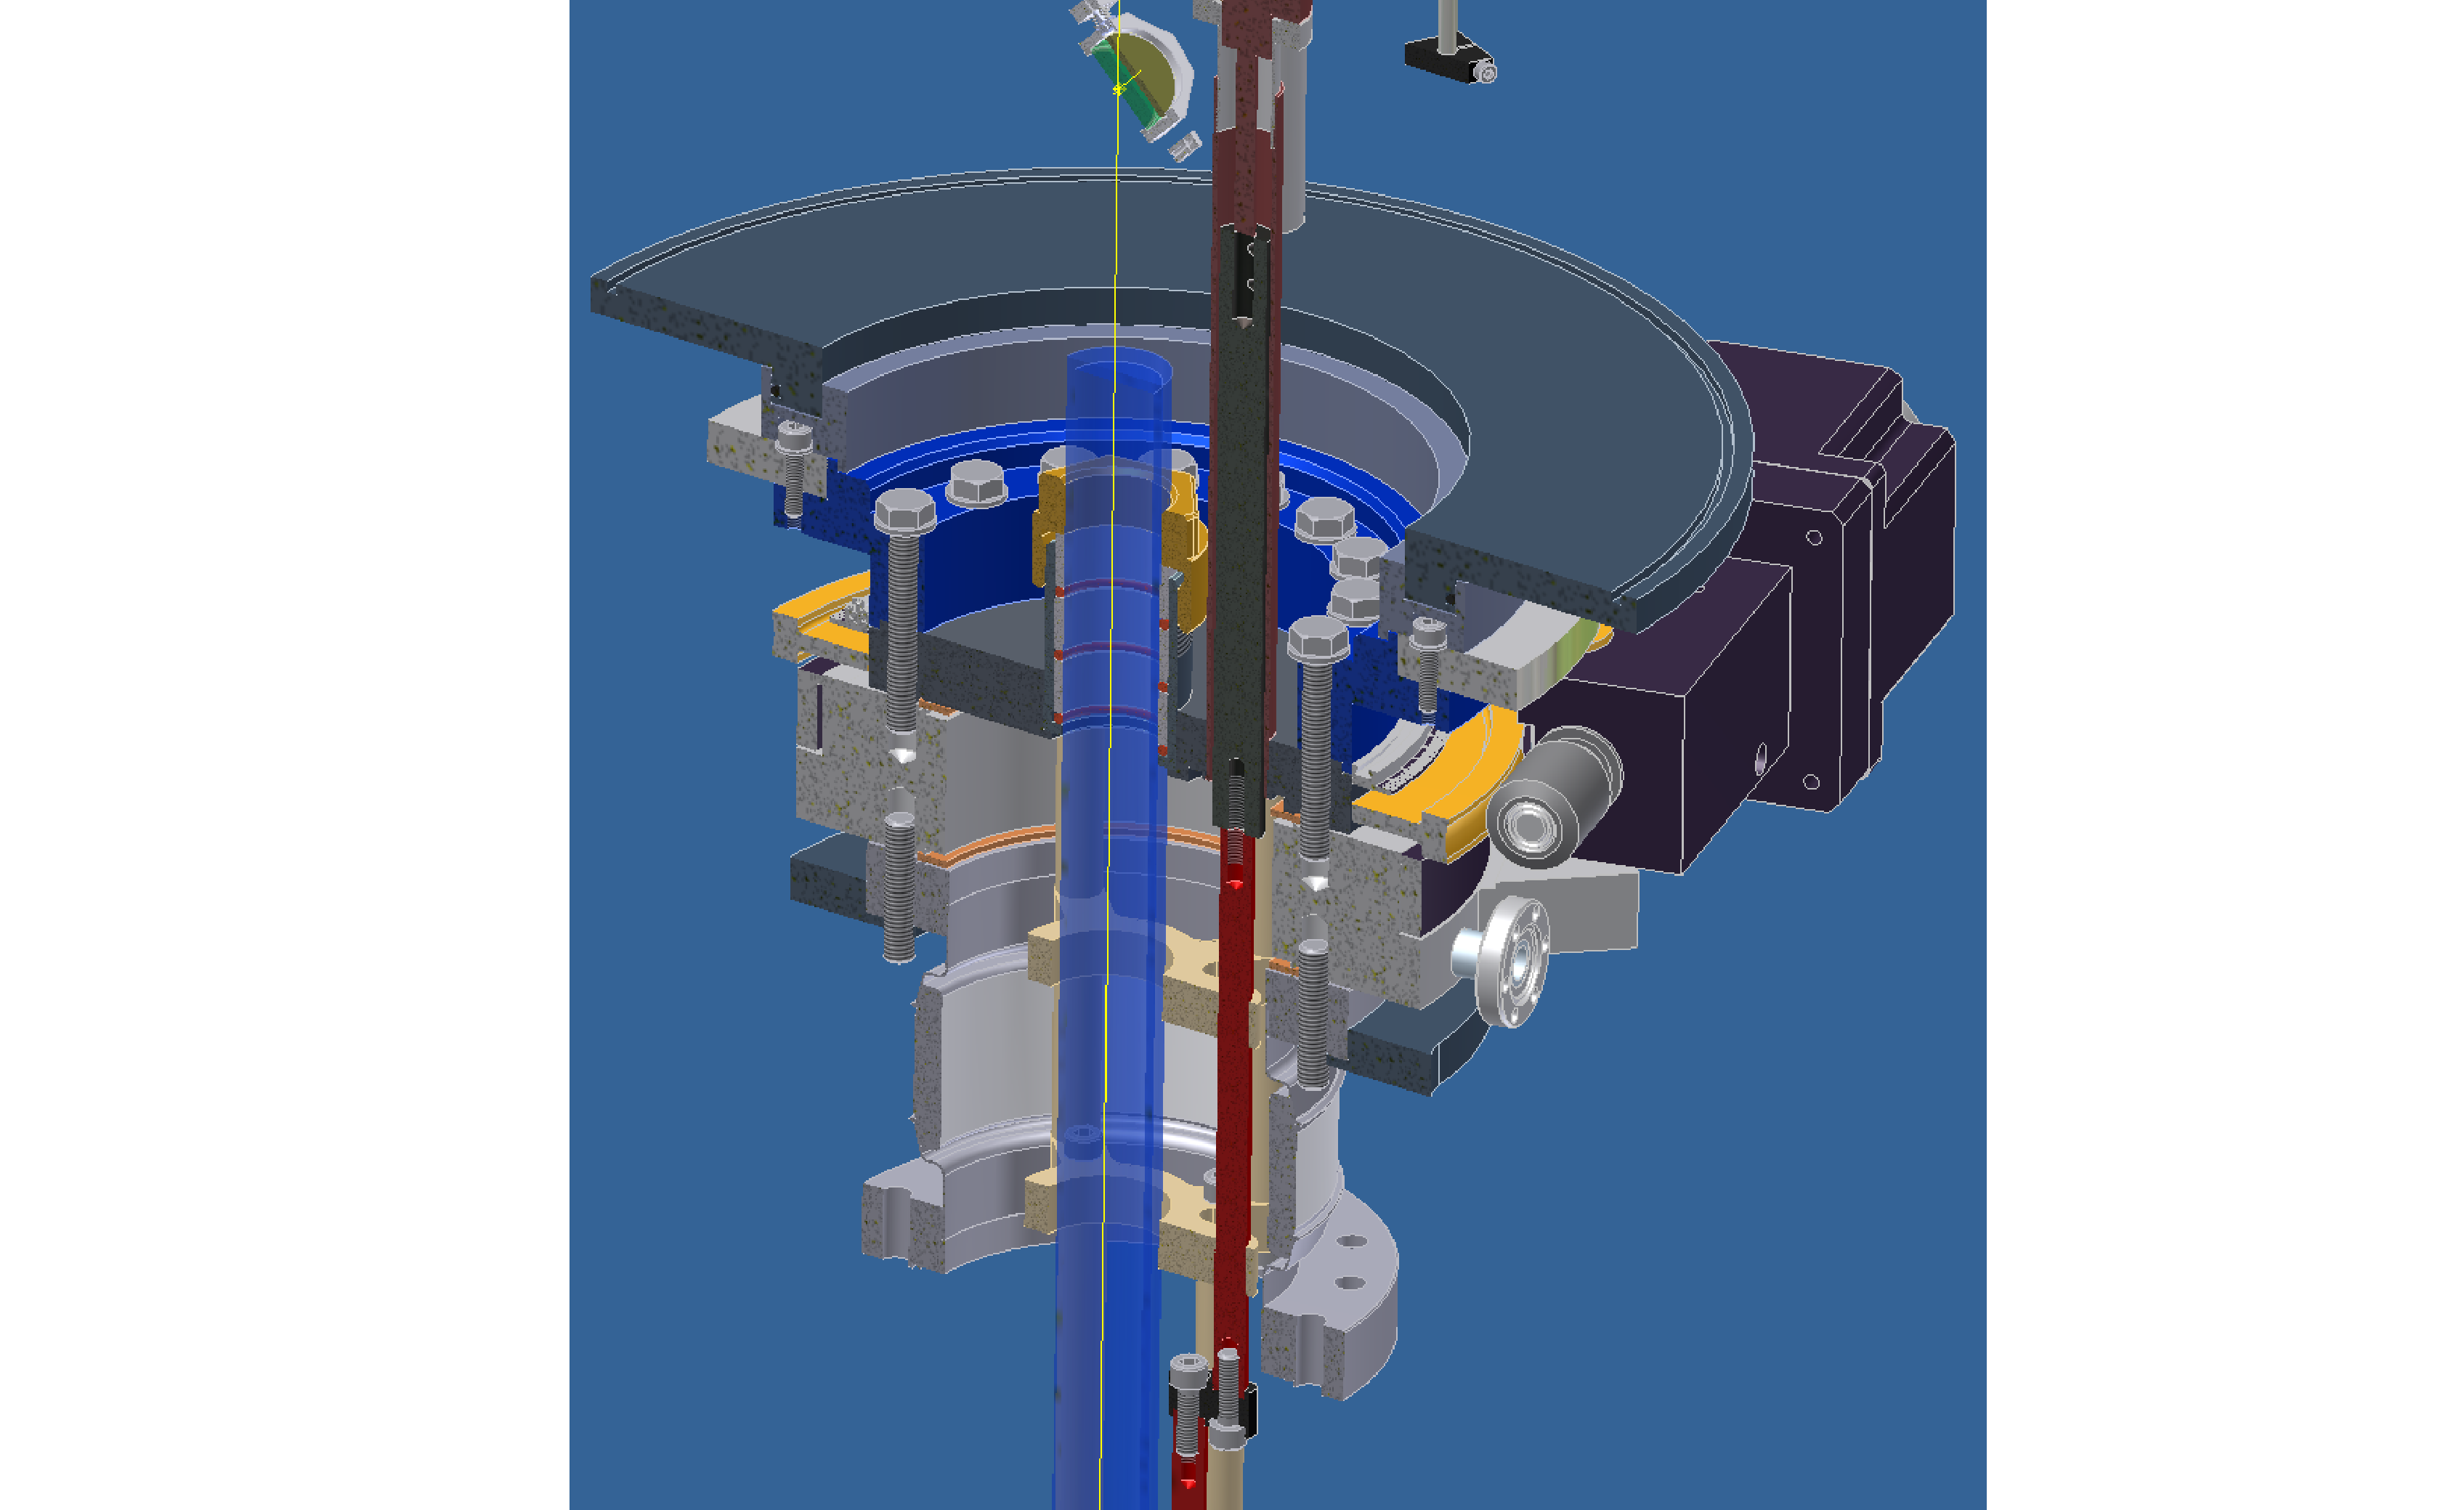
\includegraphics[height=0.6\textwidth]{figures/Feedthrough.pdf} 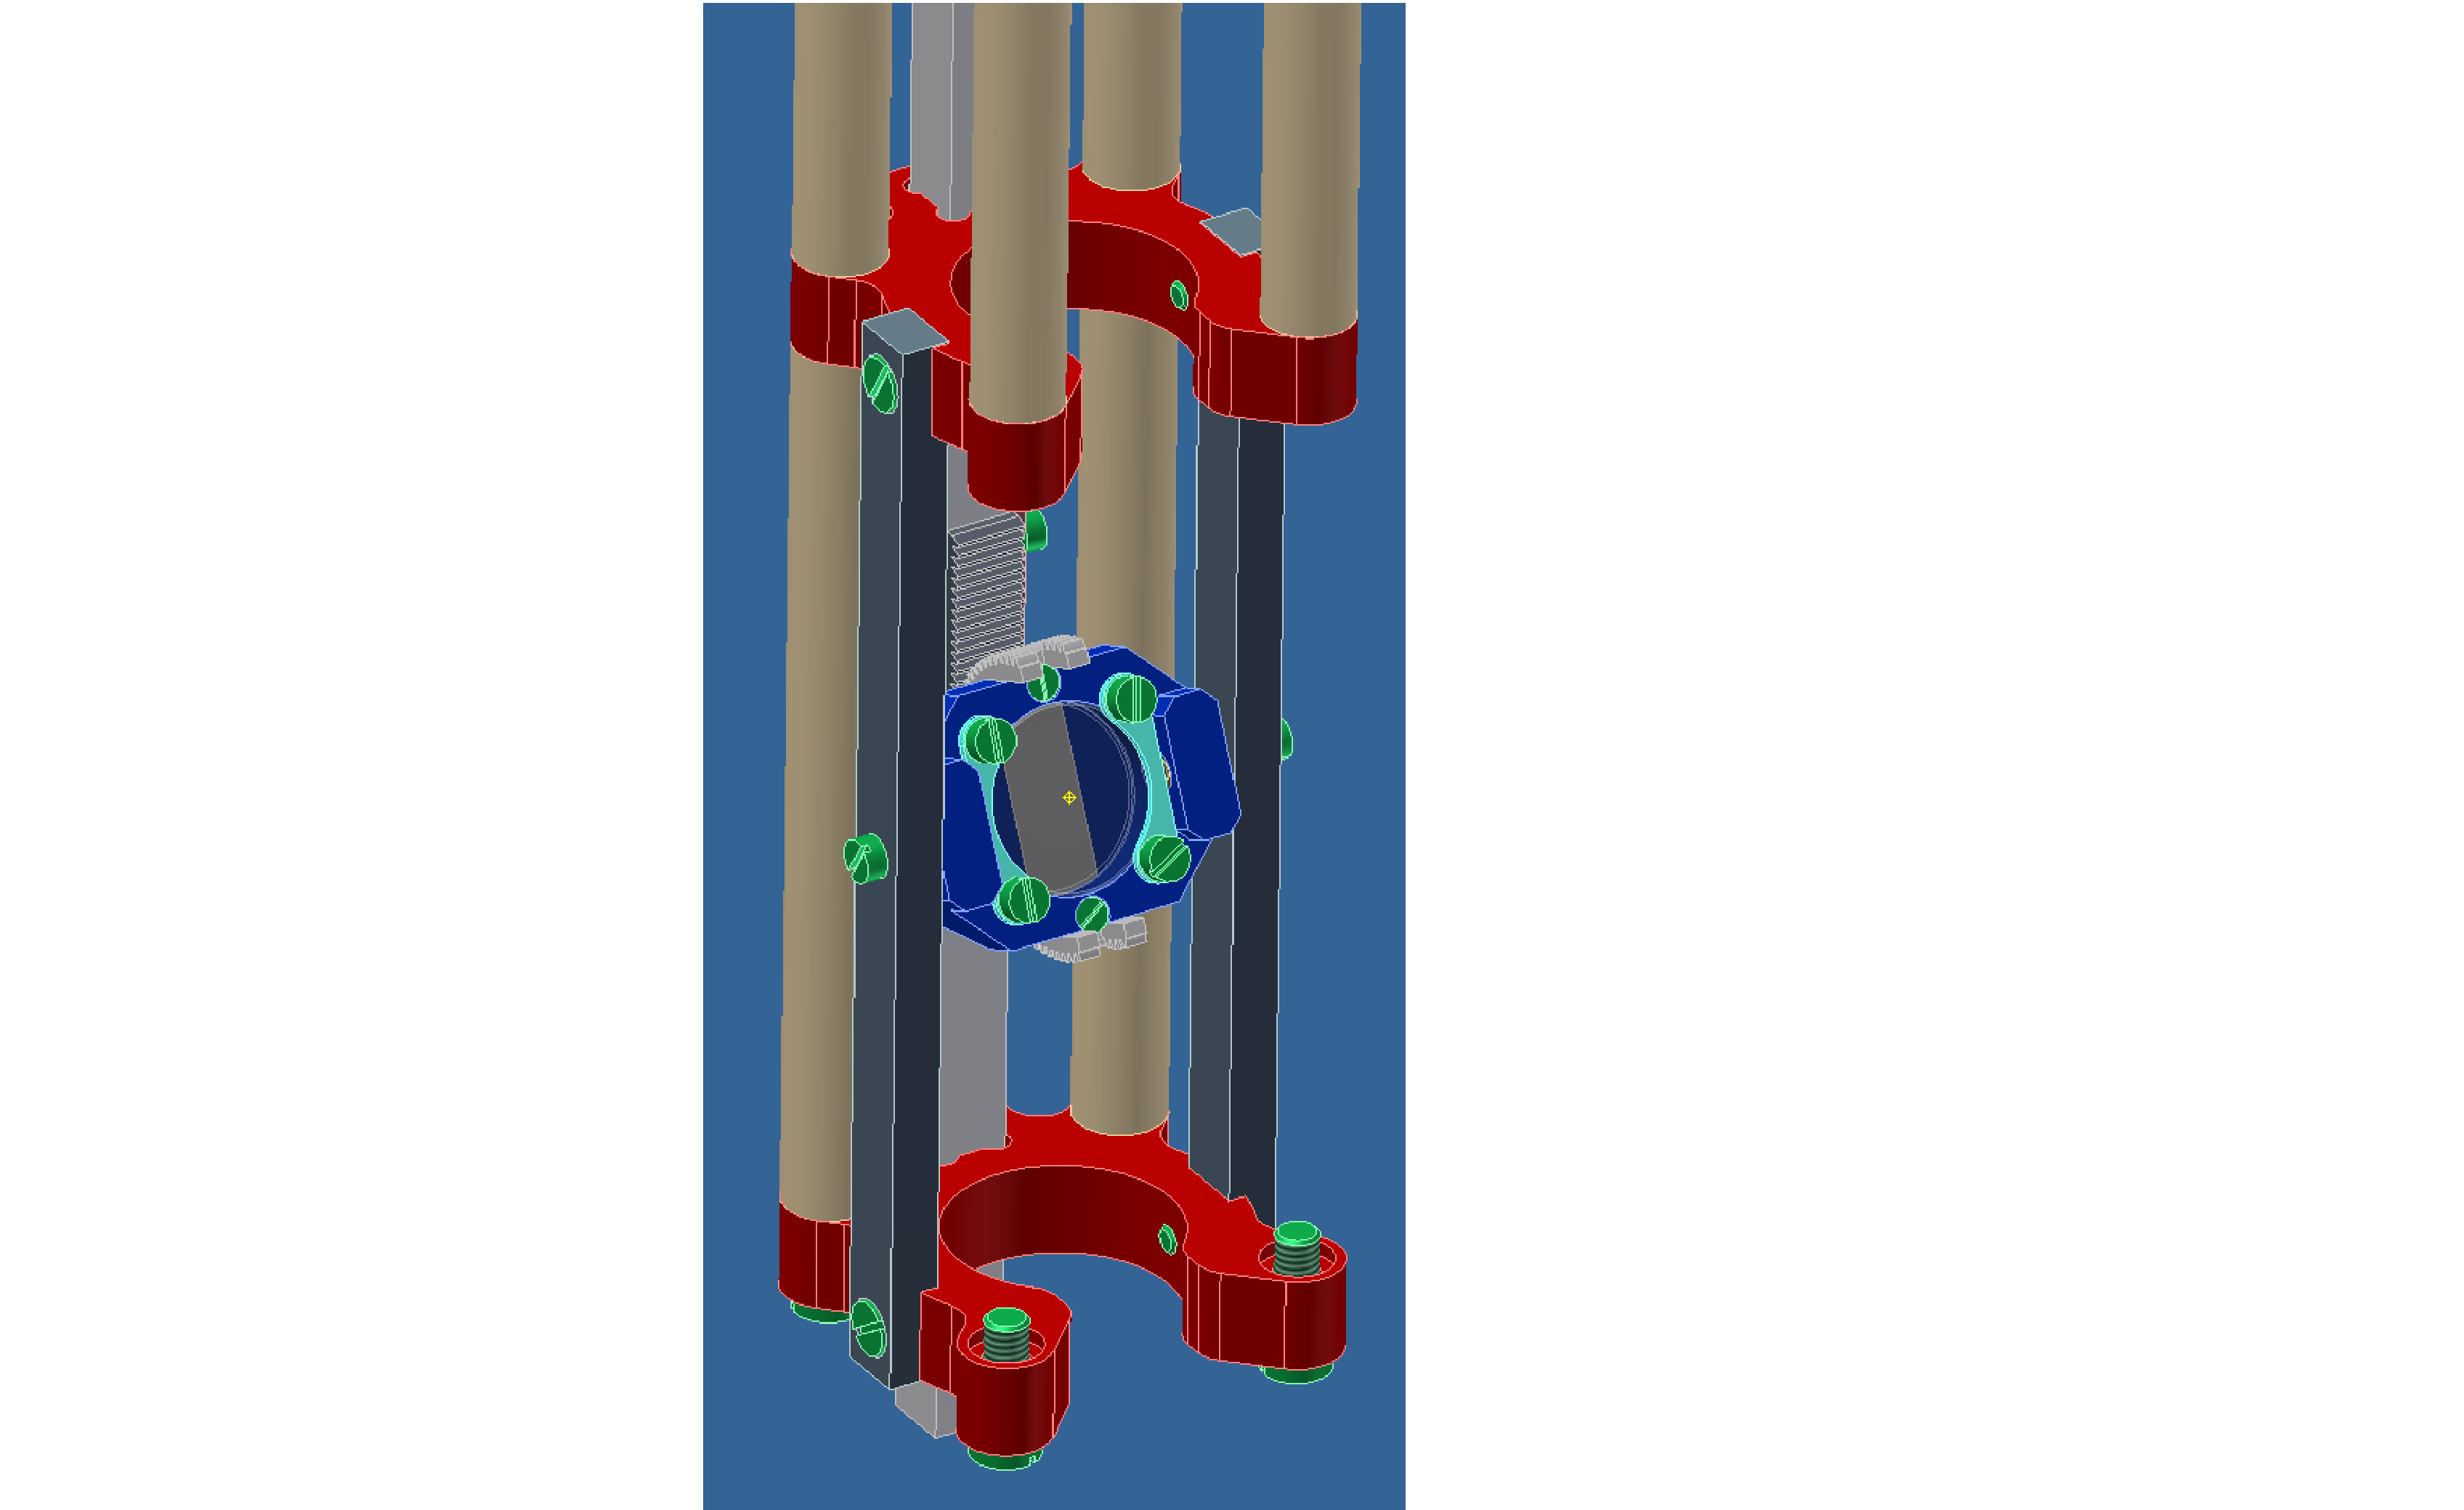
\includegraphics[height=0.6\textwidth]{figures/Mirror.pdf}
     \caption[CAD drawing of the feedthrough and the mirror support structure.]{Left: CAD cutaway drawing of the feedthrough construction is shown. The yellow line indicates the laser path. Right, CAD drawing of the cold mirror including the support structure.}
  \label{fig:feedthrough}
\end{figure}

%\begin{figure}[htb]
%\centering	
%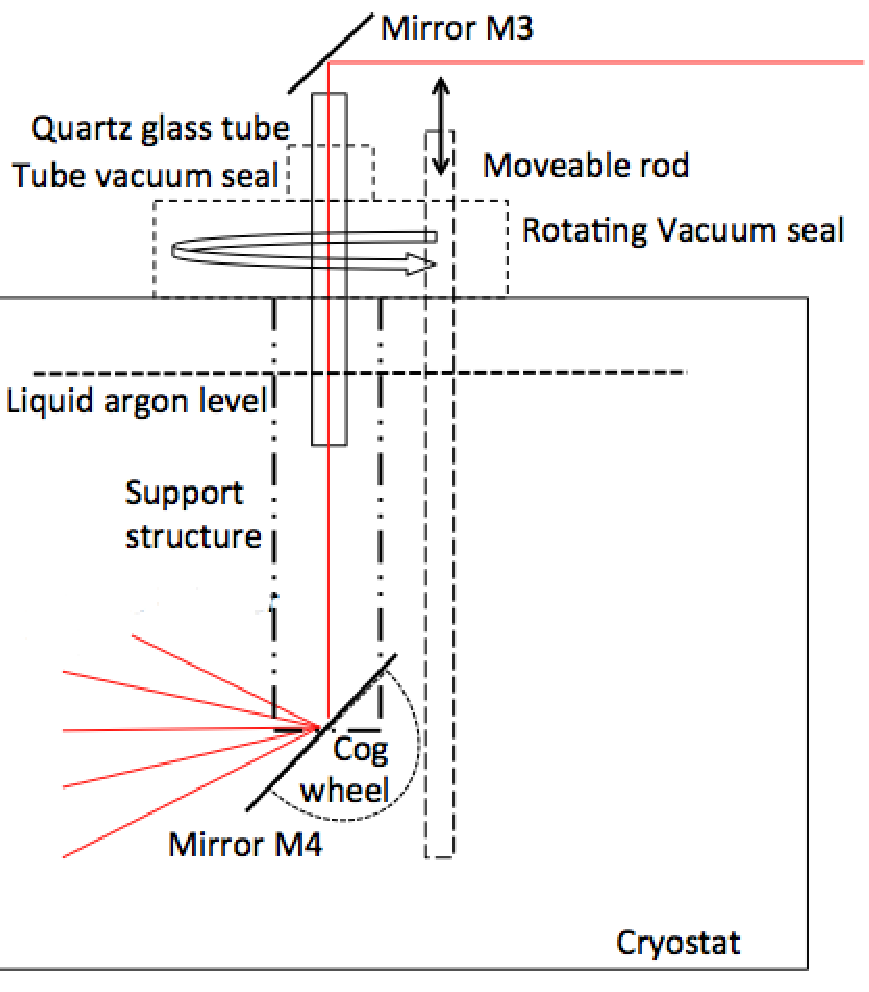
\includegraphics[width=0.8\textwidth]{figures/Arrangement-2.pdf}
%
\includegraphics[width=0.8\textwidth]{figures/temp.pdf}
%\caption{Steering of laser beams in MicroBooNE detector.}
%\label{Arrangement2}
%\end{figure}

\subsection{Performance Tests and Initial Operation}

A full performance test of the laser calibration system identical to the one installed in the MicroBooNE \lartpc was performed prior to the final installation. Apart from the general proof-of-principle of the laser calibration system, several operationally relevant parameters were identified. These include scanning speed, positioning accuracy, positioning limits, optimal laser beam intensity, beam diameter, and the minimal achievable field distortion which can be resolved. The test system consists of a \lartpc equipped with 64 readout channels and an active area of about 400 $cm^2$, with a drift distance of 40~cm (see \cite{lasertest} for further details).

Several tests of the motorized feedthrough were performed under warm conditions before cold tests were conducted. One crucial parameter for the quality of the electric field calibration is the resolution at which laser tracks can be aimed in the detector. For the rotational axis this angle is directly measured on a circular scale. For the vertical movement the linear displacement of the bellow is translated into a rotation inside the cryostat, as can be seen in the CAD drawing in figure \ref{fig:feedthrough}. This construction introduces uncertainties to the measurement position and backlash. The backlash can be compensated by always approaching positions from the same direction. For the translation of the linear movement $\Delta L$ into a rotation $\Delta \phi$ the translation ratio $s$ according to $\Delta L = s \cdot \Delta \phi$ was measured with a laser alignment device\footnote{Bosch GPL3.}.  The obtained ratio is $s=0.3499\pm 0.0002~mm/^{\circ}$. The dominant uncertainty in the vertical position measurement is the accuracy of the encoder $\sigma_{linear} = \pm 1~\mu m$, which translates into a vertical rotation measurement accuracy $\sigma_{vertical} = 10.29{''}$. 

Horizontal movement limitations arise from the construction of the feedthrough system, namely the warm mirror support structure. This limit has its origins in the way of mounting the laser table relative to the feedthrough on the MicroBooNE cryostat. Vertically the mirror can be rotated more than 45$^{\circ}$ relative to the horizon in both directions. In an upward looking configuration, no limitations arise which would affect the coverage of the detector with the beam. A limit arises when the mirror faces the opposite downward direction, when properly aligned onto the centre of the mirror the laser diameter and the size of the mirror limits the achievable coverage. However slight misalignment will affect this limit, since the beam will not be in the optimal spot anymore. In warm tests an maximal downward angle of the beam of 52.5$^{\circ}$ with respect to the horizon was achieved. During the cold tests the horizontal movement speed was set to 2.6~{$^{\circ}$/s} and the vertical speed to 1~{$^{\circ}$/s}, horizontally an angle of 81~{$^{\circ}$} was covered and 22~{$^{\circ}$} vertically, respectively. Tests in warm of the fully expanded setup showed vibrations if to high speed was chosen. The vibrations are expected to be dampened with a more stable fixation on the detector and the immersion of the setup in liquid argon.

Modulation of the beam energy with respect to the vertical alignment of the cold mirror was found to be crucial for obtaining sufficient ionization in the detector. Investigations showed that the reflectivity of the selected dielectric mirrors, which were optimized for 45$^{\circ}$ in air, are very sensitive to the angle of incidence in liquid argon. Therefore during a calibration run, the beam energy has to be controlled. The emitted UV-laser beam has a diameter of 6~mm and will spatially diverge during propagation.  A beam with this diameter will produce an ionization signal larger than the wire spacing, which will limit the capabilities of the full system. With the aperture a small as possible diameter of the laser was selected to enter the detector. Measurements of the diameter were performed with thermal paper (used for thermal printing) on which the selected beam spot burns in. The minimal achieved diameter was 1~mm.


